\documentclass[border=4pt]{standalone}
\usepackage{tikz}
\usetikzlibrary{shapes.geometric,calc,positioning,arrows.meta}

\begin{document}
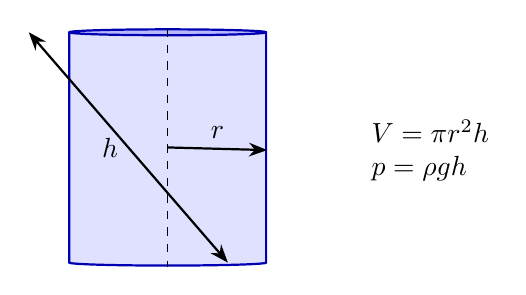
\begin{tikzpicture}[>=Stealth]
  \node[
    cylinder,
    shape border rotate=90,
    shape aspect=.32,
    draw=blue!70!black,
    line width=.8pt,
    minimum width=2.5cm,
    minimum height=3cm,
    cylinder uses custom fill,
    cylinder body fill=blue!12,
    cylinder end fill=blue!28
  ] (tank) at (0,0) {};

  \draw[<->,thick] ($(tank.before bottom)+(-5mm,0)$) --
    node[left] {$h$} ($(tank.before top)+(-5mm,0)$);
  \draw[->,thick] (tank.shape center) -- node[above] {$r$} (tank.east);
  \draw[dashed] (tank.top) -- (tank.bottom);
  \node[right=12mm of tank,align=left] {$V=\pi r^2h$\\$p=\rho gh$};
\end{tikzpicture}
\end{document}
